
\section{~Numerical approaches} \label{chapt:num}
\newcounters
\vssub
\subsection{~Basic concepts} \label{sec:basic_num}
\vssub

Equation (\ref{eq:bal_plane}) or (\ref{eq:bal_sphere}) represents the basic
equations of the wave model. However, modified versions of these equations are
used in the model, where (a) they are solved on a variable wavenumber grid
(see below), where (b) a modified versions of these equations are used to
properly described dispersion for discretized equations in selected numerical
schemes (see section~\ref{sub:xy_prop}), and where (c) sub-grid obstacles such
as islands are considered (see section~\ref{sub:xy_prop}).

If (\ref{eq:bal_plane}) or (\ref{eq:bal_sphere}) is solved directly, an
effective reduction of spectral resolution occurs in shallow water
\citep[see][]{tol:GAOS98b}. This loss of resolution can be avoided if the
equation is solved on a variable wavenumber grid, which implicitly
incorporates the kinematic wavenumber changes due to shoaling. Such a
wavenumber grid corresponds to a spatially and temporally invariant frequency
grid \citep{tol:GAOS98b}. The corresponding local wavenumber grid can be
calculated directly from the invariant frequency grid and the dispersion
relation (\ref{eq:disp}), and hence becomes a function of the local depth
$d$. To accommodate economical calculations of $S_{nl}$, a logarithmic
frequency grid is adopted,

%----------------------------%
% Logarithmic frequency grid %
%----------------------------%
% eq:sigma_grid

\begin{equation}
\sigma_{m+1} = X_\sigma \, \sigma_m \: , \label{eq:sigma_grid}
\end{equation}

\noindent
where $m$ is a discrete grid counter in $k$-space. $X_\sigma$ is defined by
the user in the input files of the program. Traditionally, in most
applications of third-generation models $X_\sigma = 1.1$ is used.

The effects of a spatially varying grid will be discussed for the Cartesian
equation (\ref{eq:bal_plane}) only. Adaptation to the spherical grid is
trivial. Denoting the variable wavenumber grid with $\kappa$, the balance
equation becomes

%------------------------------%
% general equations kappa-grid %
%------------------------------%
% eq:bal_f_grid
% eq:sigma_dot

\begin{equation}
\frac{\p}{\p t} \frac{N}{c_g} +  
\frac{\p}{\p x} \frac{\dot{x} N}{c_g} + 
\frac{\p}{\p y} \frac{\dot{y} N}{c_g} + 
\frac{\p}{\p \kappa} \frac{\dot{\kappa} N}{c_g} + 
\frac{\p}{\p \theta} \frac{\dot{\theta} N}{c_g}  =
0 \: , \label{eq:bal_f_grid} \end{equation} \begin{equation}
\dot{\kappa} \:\frac{\p k}{\p \kappa} =
     c_g^{-1} \frac{\p \sigma}{\p d} \left (
    \frac{\p d}{\p t} + {\bf U} \cdot \nabla_x d \: \right ) -
    {\bf k} \cdot \frac{\p {\bf U}}{\p s}
\: . \label{eq:sigma_dot}
\end{equation}

\noindent
Equation (\ref{eq:bal_f_grid}) is solved using a fractional step method, as is
commonplace in wave modeling. The first step considers temporal variations of
the depth, and corresponding changes in the wavenumber grid. As is discussed
by \cite{tol:GAOS98b}, this step can be invoked sparsely. By splitting off
effects of (temporal) water level variations, the grid becomes invariant, and
the depth becomes quasi-steady for the remaining fractional steps. Other
fractional steps consider spatial propagation, intra-spectral propagation and
source terms.

The multiple splitting technique results in a model that can efficiently be
vectorized and parallelized at the same time. The time splitting furthermore
allows for the use of separate partial or dynamically adjusted time steps in
the different fractional steps of the model. \ws\ makes a distinction between
4 different time steps. \label{dt_list}

\begin{list}{xx}{\itemsep 0mm \parsep 0mm \rightmargin 5mm}

\item[1)] The `global' time step $\Delta t_g$, by which the entire solution is
propagated in time, and at which intervals input winds and currents are
interpolated. This time step is provided by the user, but can be reduced
within the model to reach a requested input or output time.

\item[2)] The second time step is the time step for spatial propagation. The
user supplies a reference maximum propagation time step for the lowest model
frequency $\Delta t_{p,r}$, assuming no currents, and no grid motion. For the
frequency with counter $m$, the maximum time step $\Delta t_{p,m}$ is
calculated within the model as

%-------------------------%
% Time stepping equations %
%-------------------------%
% eq:dtpl

\begin{equation}
\Delta t_{p,m} = \frac{{\dot{x}}_{p,r}}{{\dot{x}}_{p,m}} \Delta t_{p,r}
\: . \label{eq:dtpl} \end{equation}

\noindent
where $\dot{x}_{p,r}$ is the maximum advection speed for the longest waves
without currents or grid motion, and $\dot{x}_{p,m}$ is the actual maximum
advection speed (including current) for frequency $m$. If the propagation time
step is smaller than the global time step, the propagation effects are
calculated with a number of successive smaller time steps. This generally
implies that several partial time steps are used for the lowest frequency, but
that the highest frequencies are propagated over the interval $\Delta t_g$
with a single calculation. The latter results in a significantly more
efficient model, particularly if higher-order accurate propagation schemes are
used. Note that $\Delta t_{p,m}$ may be defined bigger than $\Delta t_g$, and
that this has potential impact in model economy for cases with (strong)
currents.

\item[3)] The third time step is the time step for intra-spectral
propagation. For large-scale and deep-water grids this time step can generally
be taken equal to the global time step $\Delta t_g$. For shallow water grids,
smaller intra-spectral propagation time steps allow for larger effects of
refraction within the stability constraints of the scheme. Note that the order
of invoking spatial and intra-spectral propagation is alternated to enhance
numerical accuracy. If strong refraction o narrow swells occur, this may
result in a notable undulation of mean wave parameters. This can be avoided by
setting this time step to an even integer fraction of $\Delta t_g$.

\item[4)] The final time step is the time step for the integration of the
source terms, which is dynamically adjusted for each separate grid point and
global time step $\Delta t_g$ (see \para~\ref{sub:source}). This results in
more accurate calculations for rapidly changing wind and wave conditions, and
a more economical integration for slowly varying conditions.

\end{list}

\vspace{\baselineskip} \noindent The following sections deal with the separate
steps in the fractional step method, model input, ice treatment and boundary
data transfer between separate model grids.


% -------------------------------------------------------------
\vssub
\subsection{~Depth variations in time}
\vssub

Temporal depth variations result in a change of the local wavenumber
grid. Because the wavenumber spectrum is invariant with respect to temporal
changes of the depth, this corresponds to a simple interpolation of the
spectrum from the old grid to the new grid, without changes in the spectral
shape. As discussed above, the new grid simply follows from the globally
invariant frequency grid, the new water depth $d$ and the dispersion relation
(\ref{eq:disp}). The time step of updating the water level is generally
dictated by physical time scales of water level variations, but not by
numerical considerations \citep{tol:GAOS98b}.

The interpolation to the new wavenumber grid is performed with a simple
conservative interpolation method. In this interpolation the old spectrum is
first converted to discrete action densities by multiplication with the
spectral bin widths. This discrete action then is redistributed over the new
grid cf.\ a regular linear interpolation. The new discrete actions then are
converted into a spectrum by division by the (new) spectral bin widths. The
conversion requires a parametric extension of the original spectrum at high
and low frequencies because the old grid generally will not completely cover
the new grid. Energy/action in the old spectrum at low wavenumbers that are
not resolved by the new grid is simply removed. At low wavenumbers in the new
grid that are not resolved by the old grid zero energy/action is assumed. At
high wavenumbers in the new grid the usual parametric tail is applied if
necessary. The latter correction is rare, as the highest wavenumbers usually
correspond to deep water.

In practical applications the grid modification is usually relevant for a
small fraction of the grid points only. To avoid unnecessary calculations, the
grid is transformed only if the smallest relative depth $kd$ in the discrete
spectrum is smaller than 4. Furthermore, the spectrum is interpolated only if
the spatial grid point is not covered by ice, and if the largest change of
wavenumber is at least $0.05 \Delta k$.


% -------------------------------------------------------------
\vssub
\subsection{~Spatial propagation} \label{sub:xy_prop}
\vssub

Spatial propagation is described by the first terms of
Eq. (\ref{eq:bal_f_grid}). For the spherical grid [Eq. (\ref{eq:bal_sphere})],
the corresponding spatial propagation step becomes

%----------------------------%
% Step : Spatial propagation %
%----------------------------%
% eq:step_xy_prop

\begin{equation}
\frac{\p \cN}{\p t} + \frac{\p}{\p \phi} \, \dot{\phi} \cN +
\frac{\p}{\p \lambda} \, \dot{\lambda} \cN = 0
\: , \label{eq:step_xy_prop} 
\end{equation}

\noindent 
where the propagated quantity $\cN$ is defined as $\cN \equiv N \, c_g^{-1} \,
\cos\phi$. For the Cartesian grid, a similar equation is found propagating
$\cN \equiv N \, c_g^{-1}$. In this section equations for the more complicated
spherical grid are presented only. Conversion to a Cartesian grid is generally
a simplification and is trivial.

Equation~(\ref{eq:step_xy_prop}) in form is identical to the conventional
deep-water propagation equation, but includes effects of both limited depths
and currents. At the land-sea boundaries, wave action propagating toward the
land is assumed to be absorbed without reflection, and waves propagating away
from the coast are assumed to have no energy at the coastline. For so-called
`active boundary points' where boundary conditions are prescribed, a similar
approach is used. Action traveling toward such points is absorbed, whereas
action at the boundary points is used to estimate action fluxes for components
traveling into the model.

Three separate issues arise regarding the spatial propagation. The first is
the actual propagation scheme used (\para~\ref{sec_xypro}). The second is
the occurrence and alleviation of the Garden Sprinkler Effect (GSE) as
discussed in \para~\ref{sec_GSE}. The third is the inclusion of the effects
of unresolved obstacles on wave propagation. Sub-grid treatment of such
obstacles is addressed in \ws\ as part of the numerical propagation scheme,
and is discussed in \para~\ref{sec_obst}.


% -------------------------------------------------------------
\vsssub
\subsubsection{~Propagation schemes} \label{sec_xypro}
\vsssub

A simple and cheap first order upwind scheme has been included, mainly for
testing during development of \ws. To assure numerical conservation of action,
a flux or control volume formulation is used. The flux between grid points
with counters $i$ and $i-1$ in $\phi$-space $(\cF_{i,-})$ is calculated as

% ------ First order scheme ------- %
% eq:1up_xy_1        Basic flux
% eq:1up_xy_2        Boundary velocity
% eq:1up_xy_3        Upstream value

\begin{equation}
\cF_{i,-} = \left [ \: \dot{\phi}_b \: \cN_u \: \right ]^n_{j,l,m}
\: , \label{eq:1up_xy_1} \end{equation} \begin{equation}
\dot{\phi}_b = 0.5 \: \left ( \dot{\phi}_{i-1} + \dot{\phi}_i 
\: \right )_{j,l,m} \: , \label{eq:1up_xy_2}
\end{equation} \begin{equation}
\cN_u = \left \{ \begin{array}{ccc}
\cN_{i-1} & \mbox{for} & \dot{\phi}_b \geq 0 \\
\cN_i     & \mbox{for} & \dot{\phi}_b   <  0
\end{array} \right . \: , \label{eq:1up_xy_3}
\end{equation}

\noindent
where $j$, $l$ and $m$ are discrete grid counters in $\lambda$-, $\theta$- and
$k$-spaces, respectively, and $n$ is a discrete time step
counter. $\dot{\phi}_b$ represents the propagation velocity at the `cell
boundary' between points $i$ and $i-1$, and the subscript $u$ denotes the
`upstream' grid point. At land-sea boundaries, $\dot{\phi}_b$ is replaced by
$\dot{\phi}$ at the sea point. Fluxes between points $i$ and $i+1$
$(\cF_{i,+})$ are obtained by replacing $i-1$ with $i$ and $i$ with
$i+1$. Fluxes in $\lambda$-space are calculated similarly, changing the
appropriate grid counters and increments.  The `action density' $(\cN^{n+1})$
at time $n+1$ is estimated as

% eq:1up_xy_tot

\begin{equation}
\cN_{i,j,l,m}^{n+1} = \cN_{i,j,l,m}^n
  + \frac{\Delta t}{\Delta \phi   } \left [ \cF_{i,-} - \cF_{i,+} \right ]
  + \frac{\Delta t}{\Delta \lambda} \left [ \cF_{j,-} - \cF_{j,+} \right ]
\: , \label{eq:1up_xy_tot}
\end{equation}

\noindent
where $\Delta t$ is the propagation time step, and $\Delta \phi$ and $\Delta
\lambda$ are the latitude and longitude increments, respectively. Equations
(\ref{eq:1up_xy_1}) through (\ref{eq:1up_xy_3}) with $\cN=0$ on land and
applying Eq. (\ref{eq:1up_xy_tot}) on sea points only automatically invokes
the required boundary conditions.

Note that Eq.~(\ref{eq:1up_xy_tot}) represents a two-dimensional
implementation of the scheme, for which the norm of the actual advection
vectors needs to be used in Eq.~(\ref{eq:dtpl}). Note furthermore, that this
implies a CFL criterion for the full equation, which is generally more
stringent than that for a scheme where $\lambda$ and $\phi$ propagation are
treated separately as in the third order schemes discussed below. For a grid
with equal increments in both directions, this results in a maximum time step
that is a factor $1/\sqrt{2}$ smaller for the first order scheme than for the
third order schemes.

\vspace{\baselineskip} \noindent
Also available is the \qck\ scheme \citep{art:Leo79,art:DM82} combined with
the \ult\ \tvd\ (total variance diminishing) limiter \citep{art:Leo91}. This
is the default propagation scheme for \ws. This scheme is third-order accurate
in both space and time, and has been selected based on the extensive
intercomparison of higher order finite difference schemes for water quality
models performed by \citep[see][]{PhD:Cah,pro:FC93,tol:OMB95}. This scheme is
applied to propagation in longitudinal and latitudinal directions separately,
alternating the direction to be treated first.

In the \qck\ scheme the flux between grid points with counters $i$ and $i-1$
in $\phi$-space $(\cF_{i,-})$ is calculated as\footnote{~Fluxes $(\cF_{i,+})$
between grid points with counters $i+1$ and $i$ again are obtained by
substituting the appropriate indices.}

% ------ QUICKEST scheme ---------- %
% eq:quick_1         Basic flux
% eq:quick_2         Boundary value
% eq:quick_3         Divergence
% eq:quick_4         CFL number

\begin{equation}
\cF_{i,-} = \left [ \dot{\phi}_b \: \cN_b \: \right ]^n_{j,l,m} \: , \label{eq:quick_1}
\end{equation} \begin{equation}
\dot{\phi}_b = 0.5 \: \left ( \dot{\phi}_{i-1} + \dot{\phi}_i 
\: \right ) \: , \label{eq:quick_1a}
\end{equation}  \begin{equation}
\cN_b = \frac{1}{2} \left [ \rule[0mm]{0mm}{\baselineskip} \: 
(1+C)\cN_{i-1} + (1-C)\cN_i \: \right ] - \:
\left ( \frac{1-C^2}{6} \right ) \: {\cal CU} \: \Delta\phi^2, \label{eq:quick_2} \end{equation} \begin{equation}
{\cal CU} =  \left \{ \begin{array}{ccc}
(\: \cN_{i-2} - 2\cN_{i-1} + \cN_{i} \:)\: \: \Delta \phi^{-2}
               & \mbox{for} & \dot{\phi}_b \geq 0 \\
(\: \cN_{i-1} - 2\cN_{i} + \cN_{i+1} \:)\: \Delta \phi^{-2}
               & \mbox{for} & \dot{\phi}_b   <  0
\end{array} \right . \: , \label{eq:quick_3}
\end{equation} \begin{equation}
C = \frac{\dot{\phi}_b \: \Delta t}{\Delta \phi} 
\: , \label{eq:quick_4} \end{equation}

\noindent
where $\cal CU$ is the (upstream) curvature of the action density
distribution, and where $C$ is a \cfl\ number including a sign to identify the
propagation direction. Like the first order scheme, this scheme gives stable
solutions for $|C| \leq 1$. To assure that this scheme does not generate
aphysical extrema, it is used in combination with the \ult\ limiter. This
limiter uses the central, upstream and downstream action density (suffices
$c$, $u$ and $d$, respectively), which are defined as

% ------ ULTIMATE limiter --------- %
% eq:ult_1           Cell definition
% eq:ult_2           Nondimensional action
% eq:ult_3           Monotonic limiter
% eq:ult_4           Non-monotonic action

\begin{equation} \begin{array}{ccccc}
\cN_c = \cN_{i-1} \: , \: & \cN_u = \cN_{ i } \: , \: &
                            \cN_d = \cN_{i-2} &
                            \mbox{for} & \dot{\phi}_b \geq 0 \\
\cN_c = \cN_{ i } \: , \: & \cN_u = \cN_{i-1} \: , \: &
                            \cN_d = \cN_{i+1} &
                            \mbox{for} & \dot{\phi}_b   <  0
\end{array} \: . \label{eq:ult_1} \end{equation}

\noindent
To assess if the initial state and the solution show similar monotonic or
non-monotonic behavior, the normalized action $\tilde\cN$ is defined

\begin{equation}
\tilde\cN = \frac{\cN-\cN_u}{\cN_d - \cN_u} 
\: . \label{eq:ult_2} \end{equation}

\noindent
If the initial state is monotonic (i.e., $0 \leq \tilde\cN_c \leq 1$), the
(normalized) action at the cell boundary $\cN_b$ is limited to

\begin{equation}
\tilde\cN_c \leq \tilde\cN_b \leq 1 \:\:\: , \:\:\:
\tilde\cN_b \leq \tilde\cN_c \: C^{-1} \:\:\: . 
\label{eq:ult_3} \end{equation}
\noindent otherwise \begin{equation}
\tilde\cN_b = \tilde\cN_c 
\: . \label{eq:ult_4} \end{equation}

\noindent
An alternative scheme is necessary if one of the two grid points adjacent to
the cell boundary is on land or represents an active boundary point. In such
cases, Eqs.~(\ref{eq:1up_xy_2}) and (\ref{eq:quick_2}) are replaced by

% eq:1_vel           Boundary velocity
% eq:1_bval          Boundary value

\begin{equation}
\dot{\phi}_b = \dot{\phi}_s \: ,
\label{eq:1_vel} \end{equation} \begin{equation}
\cN_b = \cN_u \: ,
\label{eq:1_bval} \end{equation}

\noindent
where the suffix $s$ indicates the (average of) the sea point(s). This
boundary condition represents a simple first order upwind scheme, which does
not require the limiter (\ref{eq:ult_1}) through (\ref{eq:ult_4}).

The final propagation scheme, similar to Eq.~(\ref{eq:1up_xy_tot}),  becomes

% eq:uq_xy_tot

\begin{equation}
\cN_{i,j,l,m}^{n+1} = \cN_{i,j,l,m}^n +
\frac{\Delta t}{\Delta \phi} \left [ \cF_{i,-} - \cF_{i,+} \right ]
\: . \label{eq:uq_xy_tot} \end{equation}

\noindent
The scheme for propagation in $\lambda$-space is simply obtained by rotating
indices and increments in the above equations\footnote{~The `soft' boundary
treatment as described on page 31 of \cite{tol:OMB02c} is no longer available,
because it is incompatible with the advanced nesting techniques introduced in
model version \WWver.}

Note that the \uq\ scheme is implemented as alternate one-dimensional schemes,
for which the maxima of component advection speeds need to be used in
Eq.~(\ref{eq:dtpl}). For consistency, the same time steps are always used for
$\lambda$ and $\phi$ propagation for a given component.


% -------------------------------------------------------------
\vsssub
\subsubsection{~Garden Sprinkler Effect} \label{sec_GSE}
\vsssub

The \uq\ scheme is sufficiently free of numerical diffusion for the so-called
`Garden Sprinkler Effect' (GSE) to occur, i.e., a continuous swell field
disintegrates into a set of discrete swell fields due to the discrete
description of the spectrum \citep[Fig.~3c]{art:BH87}. Several GSE alleviation
methods are available in \ws.

The classical GSE alleviation method is given by \cite{art:BH87}, who derived
an alternative propagation equation for the discrete spectrum, including a
diffusive correction to account for continuous dispersion in spite of the
discrete spectral description. This correction influences spatial propagation
only, which for general spatial coordinates $(x,y)$ becomes

% ------ Correction linear dispersion --------- %
% eq:d_bal_0         Booij and Holthuijsen, 1987
% eq:Dxx
% eq:Dyy
% eq:Dxy
% eq:Dss
% eq:Dnn

\begin{equation}
\frac{\p \cN}{\p t} +
\frac{\p}{\p x} \left [ \dot{x} \cN 
           - D_{xx} \frac{\p \cN}{\p x} \right ] +
\frac{\p}{\p y} \left [ \dot{y} \cN 
           - D_{yy} \frac{\p \cN}{\p y} \right ] -
2 D_{xy} \frac{\p^2 \cN}{\p x \p y} = 0
\: , \label{eq:d_bal_0}\end{equation}  \begin{equation}
D_{xx} = D_{ss} \, \cos^2 \theta + D_{nn} \, \sin^2 \theta
\: , \label{eq:Dxx} \end{equation} \begin{equation}
D_{yy} = D_{ss} \, \sin^2 \theta + D_{nn} \, \cos^2 \theta
\: , \label{eq:Dyy} \end{equation}  \begin{equation}
D_{xy} = ( D_{ss} - D_{nn} ) \, \cos \theta \, \sin \theta
\: , \label{eq:Dxy} \end{equation} \begin{equation}
D_{ss} = (\Delta c_g )^2 \: T_s / 12
\: , \label{eq:Dss} \end{equation} \begin{equation}
D_{nn} =  ( c_g \Delta \theta )^2 \: T_s / 12
\: , \label{eq:Dnn} \end{equation}

\noindent
where $D_{ss}$ is the diffusion coefficient in the propagation direction of
the discrete wave component, $D_{nn}$ is the diffusion coefficient along the
crest of the discrete wave component and $T_s$ is the time elapsed since the
generation of the swell. In the present fractional step method the diffusion
can be added as a separate step

% eq:d_bal_1         Separated diffusion equation

\begin{equation}
\frac{\p \cN}{\p t} = 
\frac{\p}{\p x} \left [ D_{xx} \frac{\p \cN}{\p x} \right ] +
\frac{\p}{\p y} \left [ D_{yy} \frac{\p \cN}{\p y} \right ] +
   2 D_{xy} \frac{\p^2 \cN}{\p x \p y}
\: . \label{eq:d_bal_1} \end{equation}

\noindent
This equation is incorporated with two simplifications, the justification of
which is discussed in \cite{tol:OMB95}. First, the swell `age' $T_s$ is kept
constant throughout the model (defined by the user, no default value
available). Secondly, the diffusion coefficients $D_{ss}$ and $D_{nn}$ are
calculated assuming deep water

% eq:Dss_d
% eq:Dnn_d

\begin{equation}
D_{ss} = \left ( \: (X_\sigma-1) \: \frac{\sigma_m}{2 k_m} \right )^2
\: \frac{T_s}{12} \: , \label{eq:Dss_d} \end{equation} \begin{equation}
D_{nn} =  \left ( \frac{\sigma_m}{2 k_m} \Delta \theta \right )^2
\: \frac{T_s}{12} \: , \label{eq:Dnn_d} \end{equation}

\noindent
where $X_\sigma$ is defined as in Eq.~(\ref{eq:sigma_grid}). With these two
assumptions, the diffusion tensor becomes constant throughout the spatial
domain for each separate spectral component.

Equation~(\ref{eq:d_bal_1}) is solved using a forward-time central-space
scheme. At the cell interface between points $i$ and $i-1$ in $\phi$ ($x$)
space, the term in brackets in the first term on the right side of
Eq.~(\ref{eq:d_bal_1}) (denoted as $\cD_{i,-})$ is estimated as

% eq:ddif_1          Discrete diffusion 1

\begin{equation}
D_{xx} \frac{\p \cN}{\p x} \approx \cD_{i,-} =
\left . D_{xx} \; \left ( \frac{\cN_i - \cN_{i-1}}{\Delta x} \right ) \: 
\right |_{j,l,m} \: . \label{eq:ddif_1} \end{equation}

\noindent
Corresponding values for counters $i$ and $i+1$, and for gradients in
$\lambda$ ($y$) space again are obtained by rotating indices and
increments. If one of the two grid points in located on land,
Eq.~(\ref{eq:ddif_1}) is set to zero. The mixed derivative at the right side
of Eq.~(\ref{eq:d_bal_1}) (denoted as $\cD_{ij,--}$) is estimated for the grid
point $i$ and $i-1$ in $x$-space and $j$ and $j-1$ in $y$-space as

% eq:ddif_2          Discrete diffusion 2

\begin{equation}
\cD_{ij,--} = \left . \: D_{xy} 
\left ( \frac{- \cN_{i,j} + \cN_{i-1,j} +
              \cN_{i,j-1} - \cN_{i-1,j-1}}
           {0.5 ( \Delta x_j + \Delta x_{j-1} ) \: \Delta y}
              \right ) \: \right |_{l,m} 
\: . \label{eq:ddif_2} \end{equation}

\noindent
Note that the increment $\Delta x$ is a function of $y$ due to the use of the
spherical grid. This term is evaluated only if all four grid points considered
are sea points, otherwise it is set to zero. Using a forward in time
discretization of the first term in Eq.~(\ref{eq:d_bal_1}), and central in
space discretizations for the remainder of the first and second term on the
right side, the final algorithm becomes

% eq:ddif_3          Discrete diffusion 3

\begin{eqnarray}
\cN_{i,j,l,m}^{n+1} = \cN_{i,j,l,m}^n + 
\frac{\Delta t}{\Delta x} 
   \left ( \cD_{i,+} - \cD_{i,-} \right ) +
\frac{\Delta t}{\Delta y}
   \left ( \cD_{j,+} - \cD_{j,-} \right ) \nonumber \\
+ \frac{\Delta t}{4} \left ( \cD_{ij,--} + 
   \cD_{ij,-+} + \cD_{ij,+-} + \cD_{ij,++} \right )
\: . \label{eq:ddif_3} \end{eqnarray}

\noindent
Stable solutions are obtained for \citep[e.g.,][Part I section
7.1.1]{bk:Fle88}

% eq:ddif_4          Stability

\begin{equation}
\frac{D_{\max} \: \Delta t}{\min(\Delta x , \Delta y)^2}
\leq 0.5 \: , \label{eq:ddif_4} \end{equation}

\noindent
where $D_{\max}$ is the maximum value of the diffusion coefficient (typically
$D_{\max} = D_{nn}$). Because this stability criterion is a quadratic function
of the grid increment, stability can become a serious problem at high
latitudes for large scale applications. To avoid that this puts undue
constraints on the time step of a model, a corrected swell age $T_{s,c}$ is
used

% eq:Ts_cor

\begin{equation}
T_{s,c} = T_s \min \left \{ \: 1 \: , \: 
\left ( \frac{\cos(\phi)}{\cos(\phi_c)} \right )^2 \: \right \}
\: , \label{eq:Ts_cor} \end{equation}

\noindent
where $\phi_c$ is a cut-off latitude defined by the user.

\vspace{\baselineskip} \noindent 
The above diffusion is needed for swell propagation only, but is not realistic
for growing wind seas. In the latter conditions, the \uq\ scheme without the
dispersion correction is sufficiently smooth to render stable fetch-limited
growth curves \citep{tol:OMB95}. To remove minor oscillations, a small
isotropic diffusion is used for growing wave components. To assure that this
diffusion is small and equivalent for all spectral components, it is
calculated from a preset cell Reynolds (or cell Peclet) number $\cR = c_g
\Delta x D_g^{-1} = 10$, where $D_g$ is the isotropic diffusion for growing
components

% eq:Dg              Diffusion growing components

\begin{equation}
D_g = \frac{c_g \: \min(\Delta x , \Delta y)}{\cR} \: , \label{eq:Dg}
 \end{equation}

\noindent
The diffusions for swell and for wind seas are combined using a linear
combination depending on the nondimensional wind speed or inverse wave age
$u_{10} c^{-1} = u_{10} k \sigma^{-1}$ as

% eq:Xg              Linear combination for diffusion
% eq:Dss_f           Final Dss
% eq:Dnn_f           Final Dnn

\begin{equation}
X_g = \min \: \left \{ \: 1 \: , \: \max \: \left [ \: 0 \: , \:
3.3 \left ( \frac{k \, u_{10}}{\sigma} \right ) - 2.3
\: \right ] \: \right \}
 \: , \label{eq:Xg} \end{equation} \begin{equation}
D_{ss} = X_g D_g + (1-X_g) D_{ss,p}
\: , \label{eq:Dss_f} \end{equation} \begin{equation}
D_{nn} = X_g D_g + (1-X_g) D_{nn,p}
\: , \label{eq:Dnn_f} \end{equation}

\noindent
where the suffix $p$ denotes propagation diffusions as defined in
Eqs.~(\ref{eq:Dss_d}) and (\ref{eq:Dnn_d}). The constants in Eqs~(\ref{eq:Dg})
and (\ref{eq:Xg}) are preset in the model.

\vspace{\baselineskip} \noindent 
The major drawback of the above GSE alleviation method is its potential impact
on model economy as discussed in relation to Eq.~(\ref{eq:ddif_4}) and in
\cite{tol:Waves01a,tol:OMOD02b}. For this reason, two additional GSE
alleviation methods have been developed for \ws.

The first of these two methods, which represents the default for \ws, replaces
the additional diffusion step (\ref{eq:d_bal_1}) with a separate fractional
step in which direct averaging of the field of energy densities for a given
spectral component is considered. The area around each grid point over which
the averaging is performed extends in the propagation ($\bs$) and normal
($\bn$) directions as

\begin{equation}
\pm \gamma_{a,s} \: \Delta c_g \: \Delta t \: \bs \:\:\: ,
\pm \gamma_{a,n} \: c_g \Delta \theta \: \Delta t \: \bn \:\:\: , \label{eq:GSE_avg}
\end{equation}

\begin{figure} \begin{center}
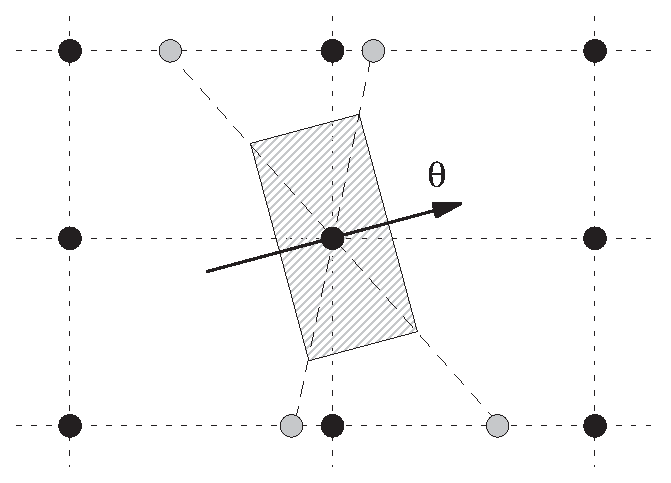
\epsfig{file=./GSE_1.eps,angle=0,width=2.2in}
\caption{Graphical depiction of spatial averaging GSE alleviation technique
used here. Solid circles and dotted lines represent the spatial grid. Hatched
area represent averaging area to be considered. Corner point values are
obtained from the central grid point and the gray points. The latter values
are obtained by interpolation from adjacent grid points
\citep[from][]{tol:OMOD02b}.}
\label{fig:GSE_1} \botline
\end{center}
\end{figure}

\noindent
where $\gamma_{a,s}$ and $\gamma_{a,n}$ are tunable constants, the default
value of which is set to 1.5. This averaging is graphically depicted in
Fig.~\ref{fig:GSE_1}. Note that these values may require some retuning for
practical applications, as discussed in \cite{tol:OMOD02b}. Appendix A of the
latter paper presents details of the averaging scheme, including conservation
considerations. Consistency with the \cite{art:BH87} approach furthermore
implies that $\gamma_{a,s}$ and $\gamma_{a,n}$ should vary with the spatial
grid resolution \citep[see][Appendix]{tol:OMOD08a}.

Note that this kind of averaging with dominant directions $\bs$ and $\bn$ is
similar to the \cite{art:BH87} diffusion method, that uses the same main
directions. The averaging method, however, never influences the time step,
because it is completely separated from the actual propagation. Moreover, if
explicit schemes are used with typically $c_g \Delta t / \Delta x < 1$, it is
obvious that the averaging over the area as defined in (\ref{eq:GSE_avg}) will
generally require information at directly neighboring spatial grid points
only, as in Fig.~\ref{fig:GSE_1}. Furthermore, this method does not require
high-latitude filtering.

As is illustrated in \cite{tol:OMOD02b,tol:OMB02b}, this method gives
virtually identical results as the previous method, but does so at slightly
lower costs. For high resolution applications, the averaging method may become
dramatically more economical.

A third possible GSE alleviation method considers that the advection for a
give discrete spectral bin is not unidirectional but divergent
\citep[see][]{tol:OMOD02b}.  An early version of this method was included in
model version 1.18. Because this method has not yet been developed to
maturity, it is not provided with the present release of \ws.

Finally, the GSE can be alleviated somewhat by assuring that the discrete
spectral directions do not coincide with spatial grid lines. This can be
achieved by defining the first discrete direction $\theta_1$ as

% eq:theta1          First direction

\begin{equation}
\theta_1 = \alpha_\theta \: \Delta \theta \:\:\: , \label{eq:theta1}
\end{equation}

\noindent
where $-0.5 \leq \alpha_\theta \leq 0.5$ can be defined by the user. Note that
setting $\alpha \neq 0$ is beneficial to the first order scheme, but has
negligible impact on the third order scheme.
 


% -------------------------------------------------------------
\vsssub
\subsubsection{~Unresolved obstacles} \label{sec_obst}
\vsssub

Even with the original tuning of \ws\ version 1.15 \citep{tol:OMB02a}, it was
clear that unresolved islands groups are a major source of local wave model
errors. This was illustrated in some more detail in
\citet[][Fig.~3]{tol:Waves01a}, and \citet[][Fig.~8]{tol:WaF02}. In \ws, a
methodology from the \swan\ model \citep{art:BRH99,man:SWAN3} was adopted to
apply the effects of unresolved obstacles at the cell boundaries of the
spatial grid within the numerical scheme. In this approach, the numerical
fluxes between cells through their common boundary are suppressed according to
the degree of obstruction provided by the unresolved obstacle. In this
approach, the numerical propagation scheme of the \uq\ scheme of
Eq.~(\ref{eq:uq_xy_tot}) is modified as

% eq:uq_xy_obstr

\begin{equation}
\cN_{i,j,l,m}^{n+1} = \cN_{i,j,l,m}^n +
\frac{\Delta t}{\Delta \phi} \left [ \alpha_{i,-} \cF_{i,-} - \alpha_{i,+} \cF_{i,+} \right ]
\: . \label{eq:uq_xy_obstr} \end{equation}

\noindent
where $\alpha_{i,-}$ and $\alpha_{i,+}$ are `transparencies' of the
corresponding cell boundaries, ranging from 0 (closed boundary) to 1 (no
obstructions). For outflow boundaries, transparencies by definition are 1,
otherwise energy will artificially accumulate in cells. For inflow boundaries,
transparencies less than 1 result in elimination of obstructed energy at the
cell boundary. This approach is graphically depicted in
Fig.~\ref{fig:obstr}. Note that a similar approach is easily adopted in the
first order scheme (\ref{eq:1up_xy_tot}). Note, furthermore, that an alternate
obstruction approach with obstructions as a function of the spectral direction
$\theta$ has been used by \cite{art:HY96} and \cite{art:HMM00}.

\begin{figure} \begin{center}
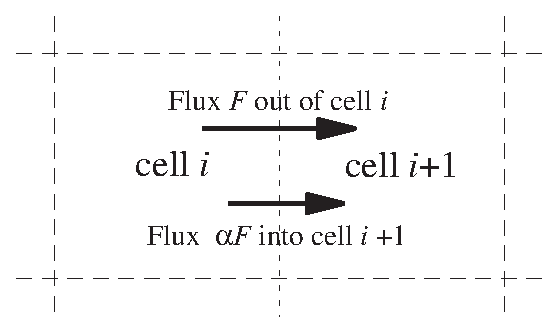
\epsfig{file=./obstr.eps,angle=0,width=2.2in}
\caption{Graphical depiction of treatment of unresolved obstacles. Common cell
         boundary (dotted line) has transparency $\alpha$. Dashed lines
         represent other cell boundaries. Numerical flux from left to right.}
         \label{fig:obstr} \botline
\end{center}
\end{figure}

Two methods for defining the obstructions are available in the model. The
first defines the obstructions directly at the grid boundary. This requires
the generation of staggered depth-transparency grids. The second allows the
user to define depths and transparencies at the same grid. In this case, the
transparency at the inflow boundary becomes $0.5(1+\alpha_i)$, and the outflow
transparency by definition is 1. To complete the total transparency
$\alpha_i$, the next cell in the flow direction will have an inflow
transparency $2\alpha_i/(1+\alpha_i)$. If consecutive cells are partially
obstructed, the product of individual transparencies is applied.

This approach can also be used to continuously model the effects of ice
coverage on wave propagation. This will be discussed in \para~\ref{sub:ice}.
Details of the sub-grid treatment of islands and ice can be found in
\cite{tol:OMOD03a}. A study of impacts of this approach in large scale wave
models is presented in \cite{tol:OMB02b,tol:OMOD03a}.

The default setting of \ws\ is not to include sub-grid modeling of
obstacles. Generating obstruction grids can be labor intensive. For this
reason, an automated approach for generating bottom and obstruction grids was
developed by \cite{tol:MMAB07a, tol:OMOD08a}.  Note that this option does not
involve compile-level choices, but is entirely controlled from the grid
preprocessor (see following chapter).


% -------------------------------------------------------------
\vsssub
\subsubsection{~Shoreline reflection \hfill {\rm (F. Ardhuin)}} \label{sec_refl}
\vsssub
In the case of  icebergs and subgrid islands, the reflected energy is redistributed evenly in all directions within 90$^\circ$ of the direction opposite to 
the incoming waves. 
For resolved lands,  a mean direction perpendicular to shore $\theta_n$ was defined 
from the land or sea status of the 8 grid points surrounding the local point (Fig. \ref{fig:refl}). 

For each model grid point adjacent to land, the analysis of the land-sea geometry gives one value of $\theta_n$  among
16 possible directions. Together with any incoming wave direction $\theta_i$ this defines a specular reflection direction $\theta_r=2 \theta_n - \theta_i + \pi$.  
For each spectral component of direction $\theta_i$ going towards the coast (i.e. such that $\cos(\theta_i-\theta_n) >0$),  the total reflection 
is $R^2$ times the incoming  energy. This reflected energy $R^2 E(f) M(f,\theta_i)$ is redistributed over directions 
around the specular reflection direction $\theta_r$, with a broad distribution taken proportional to $\cos^n(\theta-\theta_r)$, where the power $n$ 
is a function of the local shoreline geometry. 

\begin{figure} \begin{center}
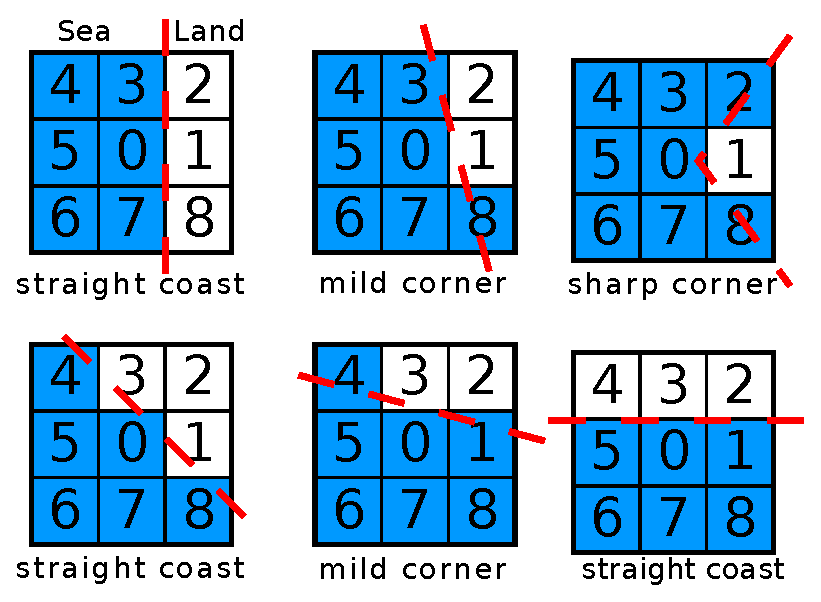
\epsfig{file=./coast_reflection.eps,angle=0,width=3in}
\caption{Examples of determination of the shoreline orientation and geometry using the land / sea mask. For any sea point (number 0) which is the ocean (in blue) 
and has at least one neighbor in land (in white) the eight neighbors, numbered from 1 to 8 are used to define the shoreline geometry. 
For `mild' corners and straight coasts, the estimated shoreline orientation (dashed line) is used to compute the directional distribution of the reflected wave energy.  
}
\label{fig:refl} \botline
\end{center}
\end{figure}

For this purpose we distinguish three different shoreline geometries relative to the local point as illustrated by 
figure \ref{fig:refl}: we set  $n=2$ for a straight coast (three connected land points 
among the neighbors), $n=1$ for a mild corner (two land points 
among the neighbors), and $n=0$ at a sharp corner (only one land point, among the 4 closest neighbors) which corresponds to the 
same treatment done for subgrid islands and icebergs. Changing these values of $n$ in the range $0$ to $2$  has little effects on our results. 
$n=1$ corresponds to a Lambertian surface approximation, which is used for electromagnetic wave scattering from rough surfaces. A pure 
specular reflection would be obtained with $n$ infinite. 
A more rigorous 
treatment should use the distribution of the shoreline orientation at at the scale of the ocean wavelength, namely of the order of 100~m. 

% -------------------------------------------------------------
\vsssub
\subsubsection{~Propagation on curvilinear grids \hfill {\rm (Rogers and Campbell)}} \label{sec_irreg}
\vsssub

Computations may be made on curvilinear grids within \ws\ . This makes it possible to run the model on alternate grid projections 
(e.g. Lambert conformal conic), rotated grids, or shoreline-following grids with higher resolution near shore, though the 
restrictions on time step from the conditionally stable schemes still apply. The same propagation schemes are utilized for 
irregular grids as for regular grids (first order upwind explicit or ULTIMATE QUICKEST).

Regarding the method: the implementation is described in \citep{RogCamp:NRLrep09}, summarized here: a Jacobian is used to convert 
the entire domain between the normal, curving space, and a straightened space. This conversion is performed only within the 
propagation routine, rather than integrating the entired model in straightened space. A simple, three step process is used every 
time the propagation subroutine is call (i.e. every time step and every spectral component): first, the dependent variable 
(wave action density) is converted to straightened space using a Jacobian; second, the wave action density is propagated via 
subroutine calls for each (of two) grid axes; third, the wave action density is converted back to normal, curved space. The actual 
flux computation is not significantly modified from its original, regular grid form. The same process occurs, regardless of grid 
type (regular or irregular); for regular grids, the Jacobian is unity.

Regarding the user interface: in {\file ww3\_grid.inp}, a string is used to indicate the grid type. In cases where this grid 
string is `{\F RECT}', the model processes input for a regular grid. In case where this grid string is `{\F CURV}' , the model 
processes input for an irregular grid. [Note that with \ws\ version 4.00, the coordinate system (i.e. degrees vs. meters) and 
the closure type (e.g. global/wrapping grid) are also specified in  {\file ww3\_grid.inp} ; the switches LLG and XYG are deprecated.] 

% -------------------------------------------------------------
\vsssub
\subsubsection{~Use of triangle-based unstructured grids \hfill {\rm (Roland and Ardhuin)}} \label{sec_prug}
\vsssub
Triangle-based grids can be used in \ws\ with numerical schemes based on contour residual distribution \citep[][for a review]{PhD:Rol}. 
This option is activated by setting the  grid string to `{\F UNST}' in {\file ww3\_grid.inp}.
Four schemes have been implemented, and the choice of one or the other is done with the UG namelist. 
These are the N scheme, the PSI scheme, the FCT scheme, and one implicit scheme. The default is the faster but more diffusive N scheme. 

In practice the grid can be easily generated, using the Polymesh interface (software developed by T.U. Darmstadt), 
from a shoreline polygons database \citep[e.g.][]{art:WS96} and a list of depth soundings, regular
or irregular. 

Regarding the method: the evolution of the spectrum at the nodes, where it is evaluated, is based on the redistribution over the nodes of
the flux convergence into the median dual cells associated with the nodes (see figure \ref{fig:triangles}).
\begin{figure} \begin{center}
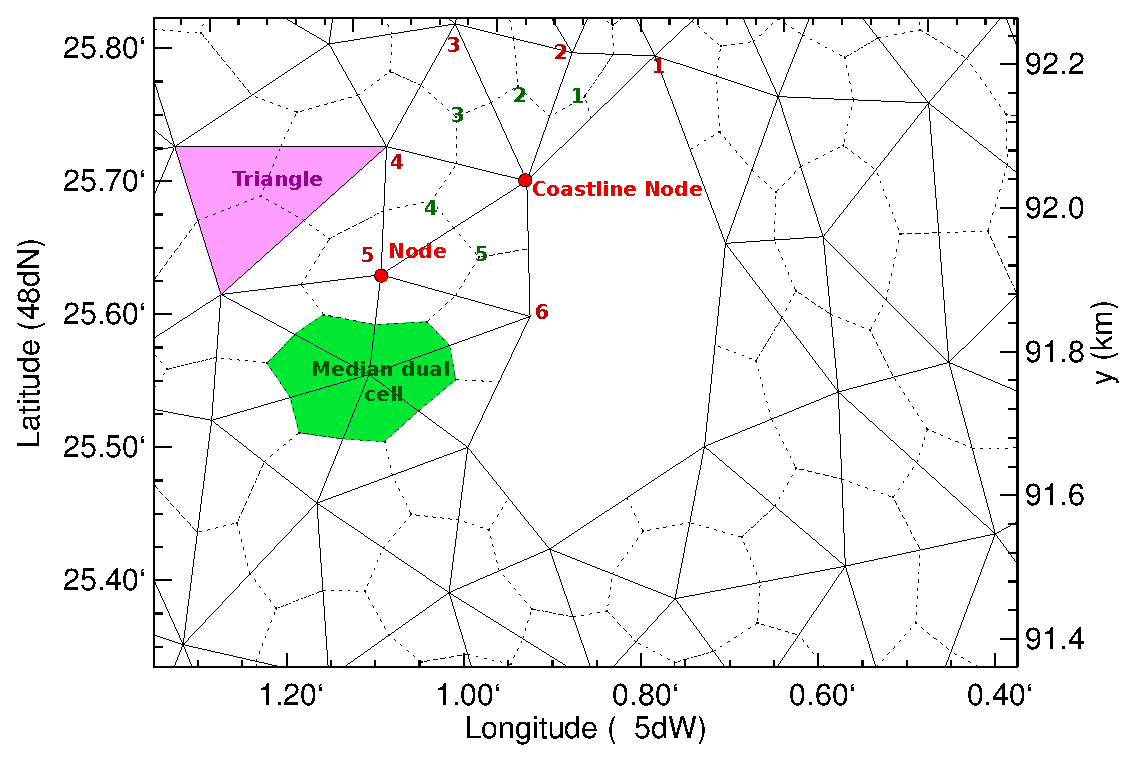
\epsfig{file=./grid_triangles.eps,angle=0,width=6in}
\caption{Example of a region of a triangle-based mesh, with in this case the small Island of Bannec, France. If the depth is greater than 
the minimum depth, the nodes of the shoreline are active. These are characterized by a larger number of neighbor nodes (6 in the example chosen) 
than neighbor triangles (5 in the same example). 
}
\label{fig:triangles} \botline
\end{center}
\end{figure}
 For any  spectral component, the advection equation (\ref{eq:step_xy_prop}) is solved on the median dwell cells: the incoming flux into a
cell gives the rate of change of the wave action at the corresponding node. The various schemes implemented have 
different discretizations for the estimation of this flux. 

 The boundary condition at the shoreline depends on the 
wave direction relative to the shoreline orientation. This particular treatment is enforced using the `{\F IOBPD}' array 
which is updated whenever the grid points status map `{\F MAPSTA}' changes. The grid geometry is also used to define 
local gradients of the water depth and currents. All other operations, such as interpolation of the forcing 
on the grid and interpolation from the grid onto output locations, is performed using linear interpolation in triangles. 

All the triangle geometry operations assume a locally flat Earth. 



% -------------------------------------------------------------
\vssub
\subsection{~Intra-spectral propagation}
\vssub

The third step of the numerical algorithm considers refraction and residual
(current-induced) wavenumber shifts. For both the spherical and Cartesian
grid, the equation to be solved in this step becomes

%-----------------------------------%
% Step : Intra-spectral propagation %
%-----------------------------------%
% eq:step_intra
% eq:k_dot_g

\begin{equation}
\frac{\p N}{\p t} + \frac{\p}{\p k} \, \dot{k}_g N +
\frac{\p}{\p \theta} \, \dot{\theta}_g N = 0
\: , \label{eq:step_intra} \end{equation} \begin{equation}
\dot{k}_g  = \frac{\p \sigma}{\p d} 
    \frac{{\bf U} \cdot \nabla_x d}{c_g}  -
    {\bf k} \cdot \frac{\p {\bf U}}{\p s}
\: . \label{eq:k_dot_g} \end{equation}

\noindent
where $\dot{k}_g$ is the wavenumber velocity relative to the grid, and
$\dot{\theta}_g$ is given by (\ref{eq:theta_g_dot}) and (\ref{eq:theta_dot}).
This equation does not require boundary conditions in $\theta$-space, as the
model by definition uses the full (closed) directional space. In $k$-space,
however, boundary conditions are required. At low wavenumbers, it is assumed
that no wave action exists outside the discrete domain. It is therefore
assumed that no action enters the model at the discrete low-wavenumber
boundary. At the high-wavenumber boundary, transport across the discrete
boundary is calculated assuming a parametric spectral shape as given by
Eq. (\ref{eq:tail_N_k}). The derivatives of the depth as needed in the
evaluation of $\dot{\theta}$ are mostly determined using central
differences. For points next to land, however, one-sided differences using sea
points only are used.

Propagation in $\theta$-space can cause practical problems in an explicit
numerical scheme, as the refraction velocity can become extreme for long waves
in extremely shallow water or due to strong current shears. Similarly, 
the propagation in $k$-space suffers from similar problems in very shallow water. 
To avoid the need of extremely small time steps
due to refraction, the propagation velocities in $\theta$-space and $k$-space
(\ref{eq:theta_dot}) are filtered,

% eq:theta_filter

\begin{equation}
\dot{\theta} = X_{rd}(\lambda,\phi,k)\left( \dot{\theta_d} + 
\dot{\theta_c} + \dot{\theta_g} \right)\: , \label{eq:theta_filter} \end{equation}

\noindent
where the indices d, c and g refer to the depth, current and great-circle related fraction of
the refraction velocity in (\ref{eq:theta_dot}). The filter factor $X_{rd}$ is
calculated for every wavenumber and location separately, and is determined so
that the \cfl\ number for propagation in $\theta$-space due to the {\em depth}
refraction term cannot exceed a pre-set (user defined) value (default
0.7). This corresponds to a reduction of the bottom slope for some low
frequency wave components. For mid-latitudes, the effected components are expected to carry
little energy because they are in extremely shallow water. Long wave
components carrying significant energy are usually traveling toward the coast,
where their energy is dissipated anyway. This filtering is also important for short waves, 
and close to the pole. The effect of this filter can be tested by reducing the time steps for
intraspectral refraction and by looking at the maximum CFL numbers in the output of the model. 
These are computed just before the filter is applied. 

\vspace{\baselineskip} \noindent 
As with the propagation in physical space, a first order and an \uq\ scheme
are available. In the first order scheme the fluxes in $\theta$- and $k$-space
are calculated Cf. Eqs. (\ref{eq:1up_xy_1}) through (\ref{eq:1up_xy_3})
(replacing $\cN$ with $N$ and rotating the appropriate counters). The complete
first order scheme becomes

% eq:1up_intra_tot

\begin{equation}
N_{i,j,l,m}^{n+1} = N_{i,j,l,m}^n 
 + \frac{\Delta t}{\Delta \theta} \left [ \cF_{l,-} - \cF_{l,+} \right ]
 + \frac{\Delta t}{\Delta k_m} \left [ \cF_{m,-} - \cF_{m,+} \right ]
\: , \label{eq:1up_intra_tot} \end{equation}

\noindent
where $\Delta \phi$ is the directional increment, and $\Delta k_m$ is the
(local) wavenumber increment. The low-wavenumber boundary conditions is
applied by taking $\cF_{m,-}=0$ for $m=1$, and the high wavenumber boundary
condition is calculated using the parametric approximation (\ref{eq:tail_N_k})
for N, extending the discrete grid by one grid point to high wavenumbers.

\vspace{\baselineskip} \noindent
The \uq\ scheme for the $\theta$-space is implemented similar to the scheme
for physical space, with the exception that the closed direction space does
not require boundary conditions. The variable grid spacing in $k$-space
requires some modifications to the scheme as outlined by
\cite[{Appendix}]{art:Leo79}. Equations~(\ref{eq:quick_1}) through
(\ref{eq:quick_4}) then become

% ------ QUICKEST scheme for k space---------- %
% eq:quick_1k        Basic flux
% eq:quick_2k        Boundary value
% eq:quick_3k        Divergence
% eq:quick_4k        CFL number

\begin{equation}
\cF_{m,-} = \left [ \dot{k}_{g,b} \: N_b \: \right ]^n_{i,j,l}
\: , \label{eq:quick_1k}\end{equation} \begin{equation}
\dot{k}_{g,b} = 0.5 \: \left ( \dot{k}_{g,m-1} + \dot{k}_{g,m} 
\: \right )  \: , \label{eq:quick_1ak}
\end{equation} \begin{equation}
N_b = \frac{1}{2} \left [ \rule[0mm]{0mm}{\baselineskip} \: 
(1+C)N_{i-1} + (1-C)N_i \: \right ] - \:
\frac{1-C^2}{6} \: {\cal CU} \: \Delta k^2_{m-1/2}, \label{eq:quick_2k} \end{equation} \begin{equation}
{\cal CU} =  \left \{ \begin{array}{ccc}
\frac{1}{\Delta k_{m-1}}
\left [ \frac{N_{ m }-N_{m-1}}{\Delta k_{m-1/2}} - 
        \frac{N_{m-1}-N_{m-2}}{\Delta k_{m,-3/2}} \right ]
               & \mbox{for} & \dot{k}_b \geq 0 \\
\frac{1}{\Delta k_m}
\left [ \frac{N_{m+1}-N_{ m }}{\Delta k_{m+1/2}} -
       \frac{N_{ m }-N_{m-1}}{\Delta k_{m-1/2}} \right ]
               & \mbox{for} & \dot{k}_b   <  0
\end{array} \right . \: , \label{eq:quick_3k}
\end{equation} \begin{equation}
C = \frac{\dot{k}_{g,b} \: \Delta t}{\Delta k_{m-1/2}}
\: , \label{eq:quick_4k} \end{equation}

\noindent
where $\Delta k_m$ is the discrete band or cell width at grid point $m$, and
where $\Delta k_{m-1/2}$ is the distance between grid points with counters $m$
and $m-1$. The \ult\ limiter can be applied as in Eqs.~(\ref{eq:ult_1})
through (\ref{eq:ult_4}), if the \cfl\ number of Eq.~(\ref{eq:quick_4k}) is
used. At the low- and high-wavenumber boundaries the fluxes again are
estimated using a first-order upwind approach, with boundary conditions as
above defined for the first-order scheme. The final scheme in $k$-space
becomes

% eq:1uq_k_tot

\begin{equation}
N_{i,j,l,m}^{n+1} = N_{i,j,l,m}^n 
 + \frac{\Delta t}{\Delta k_m} \left [ \cF_{m,-} - \cF_{m,+} \right ]
\: , \label{eq:uq_k_tot} \end{equation}


% -------------------------------------------------------------
\vssub
\subsection{~Source terms} \label{sub:source}
\vssub

Finally, the source terms are accounted for by solving

%---------------------%
% Step : Source terms %
%---------------------%
% eq:step_source

\begin{equation}
\frac{\p N}{\p t} = \cS \: . \label{eq:step_source}
\end{equation}

\noindent 
As in \wam, a semi-implicit integration scheme is used. In this scheme the
discrete change of action density $\Delta N$ becomes \citep{art:WAM88}

% eq:implicit_st

\begin{equation}
\Delta N(k,\theta) = \frac{\cS(k,\theta)}{1- \epsilon D(k,\theta)\Delta t}
\: , \label{eq:implicit_st} \end{equation}

\noindent 
where $D$ represents the diagonal terms of the derivative of $\cS$ with
respect to $N$ \citep[Eqs. 4.1 through 4.10]{art:WAM88}, and where $\epsilon$
defines the offset of the scheme. Originally, $\epsilon = 0.5$ was implemented
to obtain a second order accurate scheme. Presently, $\epsilon = 1$ is used as
it is more appropriate for the large time steps in the equilibrium range of
the spectrum \citep{pro:HA98,art:HA01}, and as it result in much smoother
integration of the spectrum. The change of $\epsilon$ has little impact on
mean wave parameters, but makes the dynamical time stepping as described below
more economical.

The semi-implicit scheme is applied in the framework of a dynamic
time-stepping scheme \citep{tol:JPO92}. In this scheme, integration over the
global time step $\Delta t_g$ can be performed in several dynamic time steps
$\Delta t_d$, depending on the net source term $\cS$, a maximum change of
action density $\Delta N_m$ and the remaining time in the interval $\Delta
t_g$. For the $n^{\rm th}$ dynamic time step in the integration over the
interval $\Delta t_g$, $\Delta t_d^n$ is calculated in three steps as

% ------ Dynamic s.t. int. scheme ------- %
% eq:st_d_1
% eq:st_d_2a
% eq:st_d_2b
% eq:st_d_3

\begin{equation}
\Delta t_d^n = 
\min_{f<f_{hf}} \left [ \frac{\Delta N_m}{|\cS|}
\left ( 1 + \epsilon D \frac{\Delta N_m}{|\cS|} \right ) ^{-1}
\right ] \: , \label{eq:st_d_1}
\end{equation} \begin{equation}
\Delta t_d^n = \max \: \left [ \: \Delta t_d^n \: , \: 
\Delta t_{d,\min} \right ] \: , \label{eq:st_d_2a}
\end{equation} \begin{equation}
\Delta t_d^n = \min \: \left [ \: \Delta t_d^n \: , \: 
\Delta t_g - \sum_{i=1}^{n-1} \Delta t_d^i
 \: \right ] \: , \label{eq:st_d_2b}
\end{equation}

\noindent
where $\Delta t_{\min}$ is a user-defined minimum time step, which is added to
avoid excessively small time steps. The corresponding new spectrum $N^n$
becomes

\begin{equation}
N^n = \max\: \left [ \: 0 \: , \: N^{n-1} + 
\left ( \frac{\cS \Delta t_d}{1 - \epsilon D \Delta t_d} \right )
\: \right ] \: . \label{eq:st_d_3}
\end{equation}

\noindent 
The maximum change of action density $\Delta N_m$ is determined from a
parametric change of action density $\Delta N_p$ and a filtered relative
change $\Delta N_r$

% eq:st_d_4
% eq:st_d_5
% eq:st_d_6
% eq:st_d_7

\begin{equation}
\Delta N_m (k,\theta) = \min \: \left [ \:
\Delta N_p (k,\theta) \: , \: \Delta N_r (k,\theta) 
\: \right ] \: , \label{eq:st_d_4}
\end{equation} \begin{equation}
\Delta N_p (k,\theta) = X_p \: \frac{\alpha}{\pi} \:
\frac{(2\pi)^4}{g^2} \: \frac{1}{\sigma k^3}
\: , \label{eq:st_d_5}
\end{equation} \begin{equation}
\Delta N_r (k,\theta) = X_r \; \max \: \left [ \: 
N(k,\theta) \: , \: N_f \: \right ] \: , \label{eq:st_d_6}
\end{equation} \begin{equation}
N_f = \max \: \left [ \: \Delta N_p (k_{\max},\theta) \: , 
\: X_f \: \max_{\forall k,\theta} \left \{ N(k,\theta) \right \}
\: \right ] \: , \label{eq:st_d_7} \end{equation}

\noindent 
where $X_p$, $X_r$ and $X_f$ are user-defined constants (see
Table~\ref{tab:st_d_p}), $\alpha$ is a {\sc pm} energy level (set to $\alpha =
0.62\,10^{-4}$) and $k_{\max}$ is the maximum discrete wavenumber. The
parametric spectral shape in (\ref{eq:st_d_5}) corresponds in deep water to
the well-known high-frequency shape of the one-dimensional frequency spectrum
$F(f) \propto f^{-5}$. The link between the filter level and the maximum
parametric change in (\ref{eq:st_d_7}) is used to assure that the dynamic time
step remains reasonably large in cases with extremely small wave energies. A
final safeguard for stability of integration is provided by limiting the
discrete change of action density to the maximum parametric change
(\ref{eq:st_d_5}) in conditions where Eq.~(\ref{eq:st_d_2a}) dictates $\Delta
t_d^n$. In this case Eq.~(\ref{eq:st_d_2a}) becomes a limiter as in the WAM
model. Impacts of limiters are discussed in detail in for instance
\cite{art:HJ99,art:HJ01}, \cite{art:HA01} and \cite{tol:GAOS02}.

% tab:st_d_p

\begin{table} 
\begin{center} \begin{tabular}{|l|c|c|c|c|} \hline \hline
                 & $X_p$     & $X_r$             & $X_f$ &
$\Delta t_{d,\min}$      \\ \hline
\wam\ equivalent & $\frac{\pi}{24}10^{-3}\Delta t$
 & $\infty (\geq 1)$ & --    & $\Delta t_g$  \\ 
 suggested       & 0.1-0.2  & 0.1-0.2 & 0.05 & $\approx 0.1 \Delta t_g$ \\  
default setting  &  0.15    &   0.10  & 0.05 & -- \\ \hline \hline
\end{tabular} \end{center}
\caption{User-defined parameters in the source term integration
 scheme}
\label{tab:st_d_p} \botline \end{table}

The dynamic time step is calculated for each grid point separately, adding
additional computational effort only for grid points in which the spectrum is
subject to rapid change. The source terms are re-calculated for every dynamic
time step.

It is possible to compile \ws\ without using a linear growth term. In such a
case, waves can only grow if some energy is present in the spectrum. In
small-scale applications with persistent low wind speeds, wave energy might
disappear completely from part of the model. To assure that wave growth can
occur when the wind increases, a so-called seeding option is available in \ws\
(selected during compilation). If the seeding option is selected, the energy
level at the seeding frequency $\sigma_{\rm seed} = \min(\sigma_{\max}, 2\pi
f_{hf})$ is required to at least contain a minimum action density

% ------ Spectral seeding ------- %
% eq:seed

\begin{eqnarray}
N_{\min}(k_{seed},\theta) & = & 
        6.25 \: 10^{-4} \frac{1}{k_{\rm seed}^3 \: \sigma_{\rm seed}}
        \max \left [ \: 0. \: , \: \cos^2 ( \theta - \theta_w ) \right ]
                             \nonumber \\ & & \hspace{5mm}
        \min \left [ \: 1 \: , \: \max \left ( \: 0 \: , \: 
        \frac{|u_{10}|}{X_{\rm seed} g \sigma_{\rm seed}^{-1}}-1 
\: \right ) \: \right ] \: , \label{eq:seed} \end{eqnarray}

\noindent
where $g \sigma_{\rm seed}^{-1}$ approximates the equilibrium wind speed for
the highest discrete spectral frequency. This minimum action distribution is
aligned with the wind direction, goes to zero for low wind speeds, and is
proportional to the integration limiter (\ref{eq:st_d_5}) for large wind
speeds. $X_{\rm seed} \geq 1$ is a user-defined parameter to shift seeding to
higher frequencies. Seeding starts if the wind speed reaches $X_{\rm seed}$
times the equilibrium wind speed for the highest discrete frequency, and
reaches its full strength for twice as high wind speeds. The default model
settings include the seeding algorithm, with $X_{\rm seed} = 1$.

In model version 3.11, surf-zone physics parameterizations have been
introduced. Such physics, particularly depth-induced breaking, operate on much
smaller time scales than deep water and limited depth physics outside the surf
zone. To assure reasonable behavior for larger time steps, an additional
optional limiter has been adopted from the SWAN model, similar to the Miche
style maximum wave height in the depth limited wave breaking source term of
Eq.~(\ref{eq:BJ78_Miche}). In this limiter, the maximum wave energy $E_m$ is
computed as

% ------ Surf zone limiter ------ %
% eq:MLIM

\begin{equation}
E_m = \frac{1}{16} [ \gamma_{lim}  \tanh ( \bar{k} d ) / \bar{k} ] ^2
\:\:\: , \label{eq:MLIM} 
\end{equation}

\noindent
where $\gamma_{lim}$ is a factor comparable to $\gamma_M$ in
Eq.~(\ref{eq:BJ78_Miche}), with the caveat that $\gamma_M$ is representative
for an individual wave, whereas $\gamma_{lim}$ is representative for the
significant wave height. For monochromatic waves, the original expression by \cite{art:Miche44} would correspond to $\gamma_{lim} = 0.94$ and
replacing $H_s$ by the height $H$ of the waves. Here this idea, is applied to random waves. 
In shallow water, this limit $H_s$ to be less than $\gamma_{lim} d$. 

If the total spectral energy $E$ is larger than the
maximum energy $E_m$, the limiter is applied by simply rescaling the spectrum
by the factor $E/E_m$, loosely following the argumentation from
\cite{art:EB96} ad used in \para\ref{sec:BJ}. This expression 

This limiter can be switch on or off in the compilation of the model, and
$\gamma_{lim}$ can be adjusted by the user. The default is set to $\gamma_{lim} =
1.6$ because $H_{rms}$ values close to $d$ have indeed been recorded and thus taking a ration 
$H_s/H_{rms}$ of 1.4, using 1.6 allows this large steepness to be exceeded by some margin. 
Note that this limiter should be used as a `safety valve' only, and
hence that it should be less strict than the breaking criterion in the
surf-breaking or whitecapping source terms, if these source terms are modeled explicitly.

Also, this limiter does not guarantee that all parts of the spectrum are realistic. Indeed, 
the use of a mean wavenumber, as in the Komen et al. dissipation, makes it possible to have unrealistically steep 
short waves in the presence of swell. A future extension of this limiter could be to limit the steepness with a partial spectral integration 
in frequencies, to make sure that waves of all scales are indeed not too steep. 


\pb
% -------------------------------------------------------------
\vssub
\subsection{~Winds and currents}
\vssub

\noindent
Model input mainly consists of wind and current fields. Within the model,
winds and currents are updated at every time step $\Delta t_g$ and represent
values at the end of the time step considered. Several interpolation methods
are available (selected during compilation). By default, the interpolation in
time consists of a linear interpolation of the velocity and the direction
(turning the wind or current over the smallest angle). The wind speed or
current velocity can optionally be corrected to (approximately) conserve the
energy instead of the wind velocity. The corresponding correction factor $X_u$
is calculated as

% eq:X_u10

\begin{equation}
X_u = \max \left [ \: 1.25 \: , \: \frac{u_{10,rms}}{u_{10,l}}
\right ] \: , \label{eq:X_u10} \end{equation}

\noindent
where $u_{10,l}$ is the linearly interpolated velocity and $u_{10,rms}$ is the
rms interpolated velocity. Finally, winds can optionally be kept constant and
changed discontinuously (option not available for current).

\vspace{\baselineskip} \noindent 
Note that the auxiliary programs of \ws\ include a program to pre-process
input fields (see \para\ref{sec:prep}). This program transfers gridded fields
to the grid of the wave model. For winds and currents this program utilizes a
bilinear interpolation of vector components. This interpolation can be
corrected to (approximately) conserve the velocity or the energy of the wind
or the current by utilizing a correction factor similar to
Eq.~(\ref{eq:X_u10}).


\pb
% -------------------------------------------------------------
\vssub
\subsection{~Use of tidal analysis \hfill {\rm (F. Ardhuin)}}
\vssub

\noindent
In order to reduce the volume of input files, the water levels and currents 
can be defined by their tidal amplitudes and phases. This is made possible 
by using the 'TIDE' switch which activates the detection of the needed 
information in current.ww3 
and level.ww3 files. The tidal analysis can be performed from NetCDF current 
or water level files, using the ww3\_prnc preprocessing program. In that case 
the analysis method uses the flexible tide analysis package by \cite{art:For09}. 
At present the choice of tidal constituents is hard coded to 20, namely, 
Z0 (mean), SSA, MSM, MSF, MF, 2N2, MU2, N2, NU2, M2, S2, K2, MSN2, MN4, M4, MS4, S4,
M6, 2MS6, and  M8. Another arbitrary choice is the time step at which currents or water 
level will be updated. This is now set to 1800~s. We also note that in the present 
version, this definition of currents and water levels can only be used with single grids, 
when using ww3\_shel. 

Memory usage and time of analysis can be greatly reduced by removing some usually negligible constituents, 
such as MSM, SSA,  MSM, 2N2, or even M8. 


% -------------------------------------------------------------
\vssub
\subsection{~Ice coverage} \label{sub:ice}
\vssub

\noindent
Ice covered sea is considered as `land' in \ws, assuming zero wave energy and
boundary conditions at ice edges are identical to boundary conditions at shore
lines. Grid points are taken out of the calculation if the ice concentration
becomes larger than a user-defined concentration. If the ice concentration
drops below its critical value, the corresponding grid point is
`re-activated'. The spectrum is then initialized with a PM spectrum based on
the local wind direction with a peak frequency corresponding to the
second-highest discrete frequency in the grid. A small spectrum is used to
assure that spectra are realistic, even for shallow coastal points.

The above discontinuous ice treatment represents the default model setting in
\ws. In the framework of the modeling of unresolved obstacles as discussed in
\para\ref{sec_obst}, a continuous method is also available, as given by
\cite{tol:OMOD03a}. In this method, a user-defined critical ice concentration
at which obstruction begins ($\epsilon_{c,0}$) and is complete
($\epsilon_{c,n}$) are given (defaults are $\epsilon_{c,0} = \epsilon_{c,n} =
0.5$, i.e., discontinuous treatment of ice). From these critical
concentrations, corresponding decay length scales are calculated as,

\begin{equation}
l_0 = \epsilon_{c,0} \min ( \Delta x , \Delta y )
\:\:\: . \label{eq:l0}
\end{equation}
\begin{equation}
l_n = \epsilon_{c,n} \min ( \Delta x , \Delta y )
\:\:\: . \label{eq:ln}
\end{equation}

\noindent
from which cell transparencies in $x$ and $y$ ($\alpha_x$ and $\alpha_y$,
respectively) are calculated as

\begin{equation}
\alpha_x = \left \{ \begin{array}{ccl}
 1 & \mbox{for} & \epsilon \Delta x < l_0 \\
 0 & \mbox{for} & \epsilon \Delta x > l_n \\
\frac{l_n - \epsilon \Delta x}{l_n - l_0} & \multicolumn{2}{c}{\mbox{otherwise}} 
\end{array} \right .
\:\:\: , \:\:\:
\alpha_y = \left \{ \begin{array}{ccl}
 1 & \mbox{for} & \epsilon \Delta y < l_0 \\
 0 & \mbox{for} & \epsilon \Delta y > l_n \\
\frac{l_n - \epsilon \Delta y}{l_n - l_0} & \multicolumn{2}{c}{\mbox{otherwise}} 
\end{array} \right .
\:\:\: . \label{eq:ice_0} 
\end{equation}

\noindent
Details of this model can be found in \cite{tol:OMOD03a}.

Updating of the ice map within the model takes place at the discrete model
time approximately half way in between the valid times of the old and new ice
maps. The map will not be updated, if the time stamps of both ice fields are
identical.


% -------------------------------------------------------------
\vssub
\subsection{~Spectral partitioning \hfill {\rm (B. Tracy)}}
\vssub

Figure \ref{fig:partitions} shows an example surface plot of an energy density
spectrum at one grid point at a specific time.  The amount of energy density
at each frequency-direction intersection is shown by this surface.  The
surface is divided into shaded areas or partitions representing energy from
sub-peaks within the spectrum.  Figure \ref{fig:partitions} shows four
spectral partitions, an area of windsea and three swell trains.  The total
energy represented by this spectrum can be defined by bulk parameters, such as
the significant wave height $H_s$. The shaded areas, called partitions of the
spectrum, show spectral sub-features that give more information about this
grid point's energy situation.  \ws\ has point and field output options
available to provide quantitative descriptions of these individual spectral
partition such as partition wave height, peak period of partition (parabolic
fit), peak wavelength of partition, mean direction of partition, wind-sea
fraction of partition ($W$) using Eq.~(\ref{eq:wsf}), and the number of
partitions.  In the field output, these parameters correspond to output fields
\ref{out:first_part} through \ref{out:last_part} and can be found in
\para\ref{sub:outpars}.

\begin{figure} \begin{center}
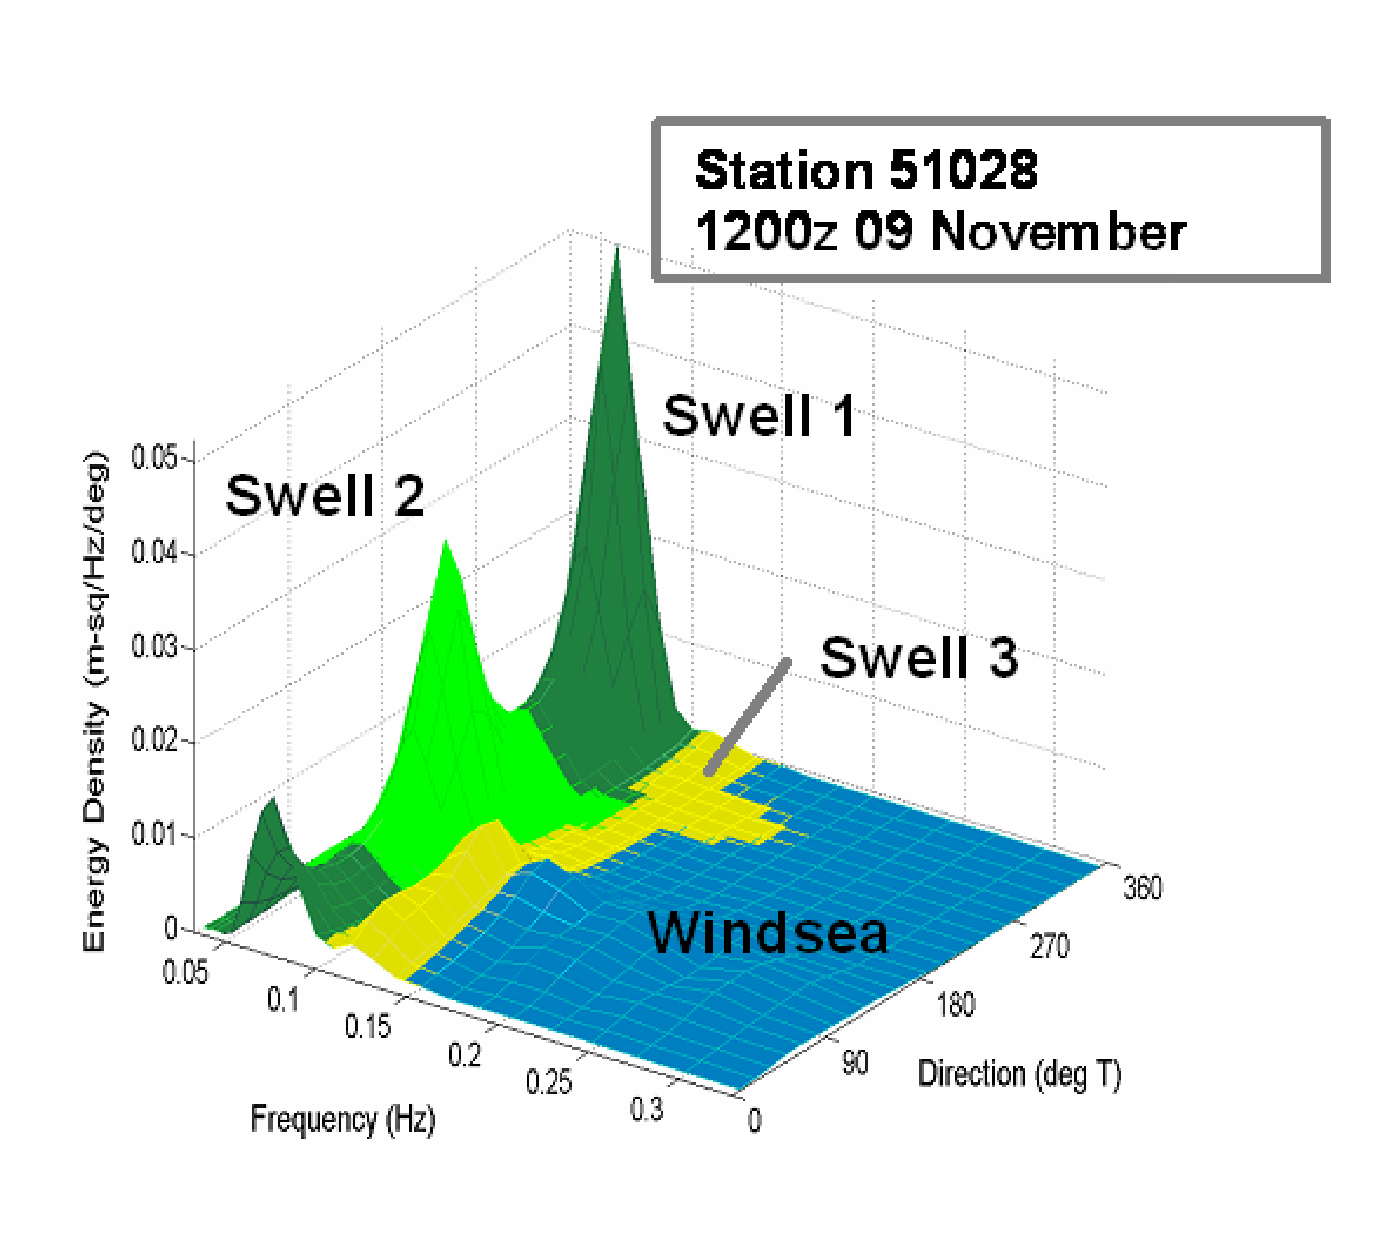
\epsfig{file=./partition.eps,width=4.0in}
\caption{Surface plot of an energy density spectrum showing spectral
         partitions for windsea and three swell trains.  This is a snapshot of
         hindcasted conditions at Christmas Island (NOAA buoy 51028) at
         12:00~UTC on November 9, 2000..}
         \label{fig:partitions} \botline
\end{center}
\end{figure}

Since the two-dimensional spectrum in Fig.~\ref{fig:partitions} looks like a
topological surface, it is logical to apply an image processing partitioning
algorithm that treats the spectral surface like a topographical surface.  The
partitioning shown in Fig.~\ref{fig:partitions} is based on a digital image
processing watershed algorithm \citep{art:VS91} first prototyped by
\cite{pro:HJ04} for the analysis of ocean wave data. The continental divide
where everything to the east goes into the Atlantic Ocean and everything to
the west goes into the Pacific Ocean is a typical example of a watershed line.
The oceans represent minima that determine the watershed line.  If the
spectral surface is inverted, the spectral peaks become catchments and
watershed lines or partition boundaries can be determined using the
\cite{art:VS91} algorithm.  Calculation of parameters for each spectral
partition can then be accomplished and wave system analysis as described in
\cite{art:HP01} can be applied.  \cite{pro:HJ04} and \cite{tol:Vict06b} used a
MATLAB code to apply the \cite{art:VS91} algorithm\footnote{~Now available as
XWaves from http://www.WaveForceTechnologies.com, replacing the previous APL
WAVES package}.  This code has been transformed to an efficient FORTRAN
routine for use in the version 3.11 of \ws.  Coding follows the
\cite{art:VS91} paper but incorporates an efficient sort routine (O(n))
discussed in \cite{rep:TTH06}.


% -------------------------------------------------------------
\vssub
\subsection{~Spatial and temporal tracking of wave systems 
\hfill {\rm (Van der Westhuysen, Hanson and Devaliere)}}
\vssub

The spectral partitioning procedure described above is carried out within 
the spectral space, independently at each geographical grid point. As a 
result, there is no coherence between the identified partitions over 
geographical space and in time. Following \cite{art:VMH97}, \cite{art:HP01} 
and \cite{pro:DHL09}, a spatial correlation step is therefore applied. 
This is done by means of an outwardly running spiral, originating at an 
arbitrary point (typically the center) inside the computational domain. 
Figure~\ref{fig:wavetrack} presents an example of such a tracking spiral on a regular 
computational grid over a coastal domain featuring landmass. At the spiral 
origin (location~1), each spectral partition is assigned an initial system 
index. The spatial correlation is then determined for each subsequent 
geographical location (2, 3, 4, ...) moving outward along the spiral. 
At each new geographical location, the peak period $T_\mathrm{p}$, peak 
direction $\theta_\mathrm{p}$ and significant wave height $H_\mathrm{m0}$ 
of each of its spectral partitions are correlated with the spatial means 
$\tilde{T}^\mathrm{n}_{\mathrm{p},i}$, $\tilde{\theta}^\mathrm{n}_{\mathrm{p},i}$ 
and $\tilde{H}^\mathrm{n}_{\mathrm{m0},i}$ of the corresponding parameters 
at its neighboring geographical grid points (indicated by the superscript 
$\mathrm{n}$) previously assigned a system $i$. the partition at the present 
grid point is assigned to the neighboring system $i$ that minimizes the 
following Goodness-of-Fit (GoF) function:

\begin{figure} \begin{center}
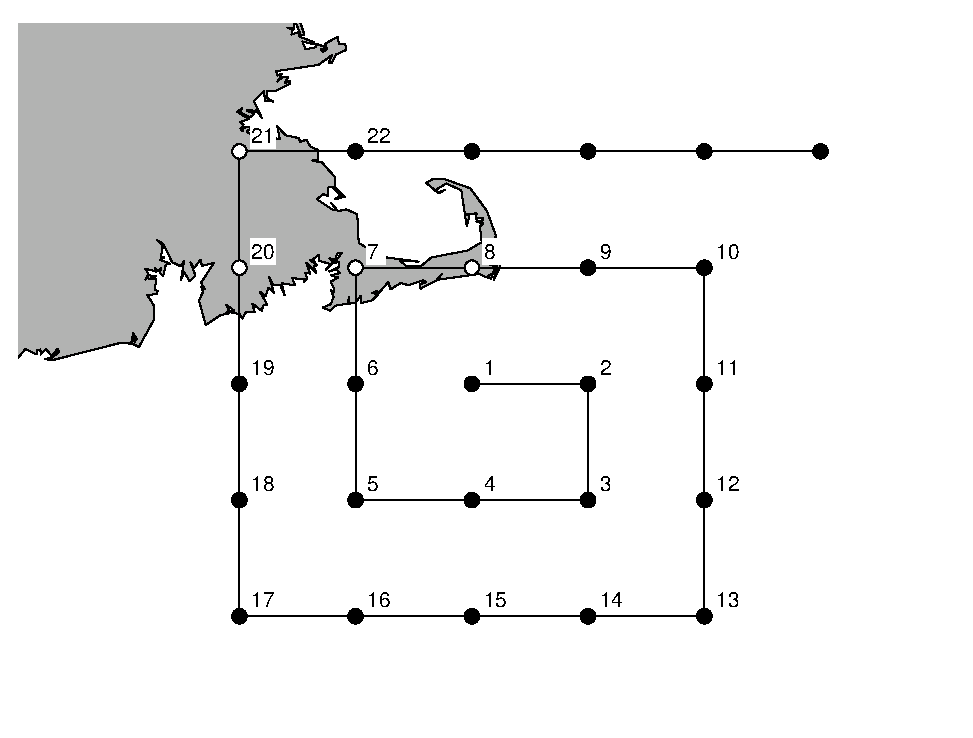
\epsfig{file=./wavetrack.eps,width=5.0in}
\caption{Example of a tracking spiral on a regular computational grid 
over a coastal domain featuring landmass (shaded). Black dots indicate 
active grid points and white dots indicate inactive (dry) grid points.}
         \label{fig:wavetrack} \botline
\end{center}
\end{figure}

\begin{equation}
    GoF_{i} = {\left( \frac{T_\mathrm{p} - \tilde{T}^\mathrm{n}_{\mathrm{p},i}}{\Delta T_\mathrm{n}} \right)}^2 + 
                     {\left( \frac{\theta_\mathrm{p} - \tilde{\theta}^\mathrm{n}_{\mathrm{p},i}}{\Delta\theta_\mathrm{n}} \right)}^2 +
                     {\left( \frac{H_\mathrm{m0} - \tilde{H}^\mathrm{n}_{\mathrm{m0},i}}{\Delta H_\mathrm{n}} \right)}^2\ \ ,
\label{eq:grdgof}
\end{equation} 

where $\Delta T_\mathrm{n}$, $\Delta\theta_\mathrm{n}$ and $\Delta H_\mathrm{n}$ 
are combining criteria, see \cite{art:WHD13}. If either of 
the first two terms on the RHS of (\ref{eq:grdgof}) exceed unity for the 
closest match, the difference is considered too great and a new wave system 
is assigned to that partition. Here, the search range for neighboring 
points is set at 1, so that a maximum of four previously-associated 
neighbors can be found (e.g. location 15 will have the previously processed 
neighbors 3, 4, 5 and 14). In some cases, iterative combining is required.

The next step is to correlate these wave systems over time. Each system 
$i$ at the current time level $t$ is associated with its closest match 
amongst the systems $j$ at the previous time level $(t-1)$. Three 
characteristics of the wave systems are considered in this process, 
namely: (i) the spatial mean peak wave period over the system, 
$\tilde{T}^\mathrm{s}_{\mathrm{p},t,i}$, with $\mathrm{s}$ denoting the 
system mean, (ii) the spatial mean peak wave direction, 
$\tilde{\theta}^\mathrm{s}_{\mathrm{p},t,i}$ and (iii) the number of 
overlapping grid points between the two systems in geographical space 
$\cap_{i,j}$. These characteristics are combined to form the following 
GoF function:

\begin{equation}
    GoF_{i,j} = {\left( \frac{\tilde{T}^\mathrm{s}_{\mathrm{p},t,i} - \tilde{T}^\mathrm{s}_{\mathrm{p},t-1,j}}{\Delta T_\mathrm{s}} \right)}^2 + 
                       {\left( \frac{\tilde{\theta}^\mathrm{s}_{\mathrm{p},t,i} - \tilde{\theta}^\mathrm{s}_{\mathrm{p},t-1,j}}{\Delta\theta_\mathrm{s}} \right)}^2 +
                       {\left( \frac{N_{t-1,j} - \cap_{i,j}}{0.5N_{t-1,j}} \right)}^2\ \ ,
\label{eq:timegof}
\end{equation} 

where $\Delta T_\mathrm{s}$ and $\Delta\theta_\mathrm{s}$ are combining 
criteria, and $N$ is the total number of grid points in a system, see 
\cite{art:WHD13}. In order to focus the tracking process on 
high-energy regions in the wave field, the spatial mean period and peak 
direction values of each system are weighted with the square of the 
significant wave height. System $i$ at the current time level $t$ is 
assigned the system $j$ from the previous time level $(t-1)$ that minimizes 
(\ref{eq:timegof}). If any of the three terms on the RHS of (\ref{eq:timegof}) 
exceed unity for the system that minimizes (\ref{eq:timegof}), a new system 
number is assigned. For the last term, this implies a minimum spatial 
overlap requirement, arbitrarily set at 50\%. This term mostly has an 
impact over basin scale domains, where systems are typically smaller than 
the computational area. In order to improve robustness, the details of 
identified systems are stored for five time levels, after which the system 
association is released.


% -------------------------------------------------------------
\vssub
\subsection{~Nesting}
\vssub

Traditionally, wave models only consider one-way nesting, with boundary data
from low resolution grids being provided to high resolution grids. This
approach has always been available in \ws, and is discussed in
\para\ref{sub:one_way}. In model version \WWver, a multi-grid wave model
driver was introduced, considering full two-way nesting between grids. This
approach is discussed in \para\ref{sub:two_way}.


% -------------------------------------------------------------
\vssub
\subsubsection{~Traditional one-way nesting} \label{sub:one_way}
\vssub

The conventional wave model program {\file ww3\_shel} considers a single wave
model grid. This program includes options to transfer boundary conditions from
large-scale runs to small-scale runs. Each run can simultaneous accept one
data set with boundary conditions, and generate up to 9 data sets with
boundary conditions. To assure conservation of wave energy with incompatible
depths and currents, the boundary data consists of energy spectra
$F(\sigma,\theta)$. The data file consists of spectra at grid points of the
generating run, and information needed to interpolate spectra at the requested
boundary points. The size of the transfer files is thus minimized if the input
points for a small-scale run are located on grid lines in the large-scale
run. When used as input, the spectra are interpolated in space and time for
every global time step $\Delta t_g$, using a linear interpolation of spectral
components. 

The numerical approach for including boundary data in a wave model is
illustrated in Fig.~\ref{fig:nest1}. Active boundary points are assigned in
the grid to separate sea points from land points or from otherwise deactivated
grid points. Between the active boundary points and sea points, a local
boundary scheme is applied (typically first order). In the internal sea points
of the model, the selected propagation scheme is used.

Practical aspect of the conventional one-way nesting approach are
discussed in more detail in Appendix~\ref{app:nest}.

\begin{figure}
\begin{center}

\setlength{\unitlength}{0.001in}

\begin{picture}(3000,1800)(0,-1550)

\put(0200,-1200){\vector(1,0){2100}}
\put(2400,-1250){\makebox(400,100){\small space}}
\put(0300,-1300){\vector(0,1){1300}}
\put(0100, 0100){\makebox(400,100)[c]{\small time}}

\multiput(0300,-1200)(0,300){4}{\circle {50}}
\multiput(0600,-1200)(0,300){4}{\circle {50}}
\multiput(0900,-1200)(0,300){4}{\circle {50}}
\multiput(1200,-1200)(0,300){4}{\circle*{50}}
\multiput(1500,-1200)(0,300){4}{\circle {50}}
\multiput(1800,-1200)(0,300){4}{\circle {50}}
\multiput(2100,-1200)(0,300){4}{\circle {50}}

\put(0300,-0150){\makebox(600,100)[c]{`land'}}
\put(0900,-0200){\vector(-1,0){575}}

\put(1500,-0150){\makebox(600,100)[c]{sea}}
\put(1500,-0200){\vector(1,0){875}}
				       
\put(0900, 0050){\makebox(600,100)[c]{bound. data}}
\put(1100,-1200){\dashbox{50}(0200,1150){}}

\put(1050,-1550){\makebox(600,100)[c]{bound. scheme}}
\put(1200,-1400){\dashbox{25}(0300,1100){}}

\put(1550,-0750){\makebox(600,100)[l]{internal scheme}}
\put(1500,-0800){\vector(1,0){875}}

\end{picture}
\end{center}

\caption{Traditional one-way nesting approach as used in {\file ww3\_shel}.
         One-dimensional representation in space and time, symbols represent
         grid points.} \label{fig:nest1}
\botline
\end{figure}



% -------------------------------------------------------------
\vssub
\subsubsection{~Two-way nesting} \label{sub:two_way}
\vssub

Model version \WWver\ introduces the multi-grid or mosaic approach to wave
modeling with the introduction of the wave model program {\file ww3\_multi}
\citep{tol:Vict06a, tol:MMAB07b, tol:OMOD08b}. In this program, an arbitrary
number of grids with arbitrary resolutions is considered, with data exchange
between grids at each relevant model time step. The grids are given a rank
number, where lower rank corresponds to lower resolution, and equal rank
corresponds to similar resolution (but not necessarily equal resolution).
Three types of data transfer between grids are considered. These are

\begin{itemize}
\item Transfer of data from lower to higher rank grids.
\item Transfer of data from higher to lower rank grids.
\item Transfer of data between grids with equal rank.
\end{itemize}

Data transfer from lower to higher ranked grids is accomplished by providing
boundary data to the higher ranked grid, as in the traditional one-way nesting
approach described in the previous section and in Fig.~\ref{fig:nest1}.

When this approach is combined with data transfer from higher to lower rank, a
full two way nesting approach is established. In {\file ww3\_multi} the data
at the lower ranked grids is reconciled with the data at the higher ranked
grids after the higher ranked grids have `caught up' in time with the lower
ranked grids.  Considering that the resolution of the lower ranked grid by
definition is lower that the resolution of the higher ranked grid, a natural
way to estimate the wave energy in the lower ranked grid $E_{l,i}$ from energy
in the higher ranked grid $E_{h,j}$ is

\begin{equation}
E_{l,i} = \sum w_{i,j} W_{h,j} \:\:\: , \label{eq:nest_hg1}
\end{equation}

\noindent
where $i$ and $j$ are grid counters in the two grids, and where $w_{i,j}$ are
averaging weights. The weights can be defined consistent with conservation of
wave energy as the surface of the grid box $j$ in the higher ranked grid that
covers the grid box $i$ in the lower ranked grid, normalized with the surface
of the lower ranked grid box $i$. This is illustrated in Fig.~\ref{fig:nest2}.
To avoid circular reconciliation, grid points in the lower ranked grid that
contribute to the boundary data in the higher ranked grid are not updated in
this manner.

\begin{figure}
\begin{center}

\setlength{\unitlength}{0.001in}

\begin{picture}(3000,1900)(0,-1600)

\multiput(0300,-1400)(0,300){6}{\circle {50}}
\multiput(0600,-1400)(0,300){6}{\circle {50}}
\multiput(0900,-1400)(0,300){6}{\circle {50}}
\multiput(1200,-1400)(0,300){6}{\circle {50}}
\multiput(1500,-1400)(0,300){6}{\circle {50}}
\multiput(1800,-1400)(0,300){6}{\circle {50}}
\multiput(2100,-1400)(0,300){6}{\circle {50}}
\multiput(2400,-1400)(0,300){6}{\circle {50}}
\multiput(2700,-1400)(0,300){6}{\circle {50}}

\multiput(0450,-1550)(300,0){8}{\dashbox{50}(0000,1800){}}
\multiput(0150,-1250)(0,300){5}{\dashbox{50}(2700,0000){}}

\multiput(0400,-1450)(0,800){3}{\circle*{100}}
\multiput(1400,-1450)(0,800){3}{\circle*{100}}
\multiput(2400,-1450)(0,800){3}{\circle*{100}}

\put(895,-1055){\framebox(1010,810){}}
\put(900,-1050){\framebox(1000,800){}}
\put(905,-1045){\framebox(990,790){}}

\end{picture}
\end{center}

\caption{Concept for reconciling lower ranked grid with higher ranked grid in
         two-way nesting approach. $\circ$ and hashed lines represent the
         higher ranked grid points and grid boxes, respectively, $\bullet$ and
         solid lines represent lower ranked grid and central grid box.}
\label{fig:nest2}
\botline
\end{figure}


Overlapping grids with similar rank cannot use the above two-way nesting
technique to consistently exchanger data. Instead, all such grids are
propagated one time step, after which the grids are reconciled as is
illustrated in Fig.~\ref{fig:nest3} For grid 1 ($\circ$ in
Fig.~\ref{fig:nest3}) two areas can be distinguished. In area C, the influence
of the boundary has propagated into the grid since the last
reconciliation. The actual depth of penetration depends on the stencil width
of the numerical scheme, and the number of propagation time steps.  In areas A
and B, information from the boundary has not yet penetrated, and this area can
be considered as the `interior' of grid 1.  Similarly, area A represents the
boundary penetration depth for grid 2 ($\bullet$ in Fig.~\ref{fig:nest3})
whereas B and C represent the interior of grid 2.  A simple and consistent
reconciliation between grid 1 and 2 uses data from grid 1 exclusively in area
A (interpolating data from grid 1 to grid points in grid 2 as necessary), and
uses data from grid 2 exclusively in area C. In area B, where interior parts
of both grids overlap, a consistent solution can be found by using weighted
averages from both grids. Note that this approach is easily extended to
multiple overlapping grids.

Note that for explicit numerical propagation schemes and overlapping grids with
identical resolution and coinciding grid points, solutions for overlapping
grids and the compatible single grid can be identical, as long as the overlap
areas are sufficiently wide.

\begin{figure}
\begin{center}

\setlength{\unitlength}{0.001in}

\begin{picture}(3000,1900)(0,-1600)

\multiput(0300,-1400)(0,300){5}{\circle {50}}
\multiput(0600,-1400)(0,300){5}{\circle {50}}
\multiput(0900,-1400)(0,300){5}{\circle {50}}
\multiput(1200,-1400)(0,300){5}{\circle {50}}
\multiput(1500,-1400)(0,300){5}{\circle {50}}
\multiput(1800,-1400)(0,300){5}{\circle {50}}
\multiput(2100,-1400)(0,300){5}{\circle {50}}

\multiput(0950,-1275)(0,300){5}{\circle*{50}}
\multiput(1250,-1275)(0,300){5}{\circle*{50}}
\multiput(1550,-1275)(0,300){5}{\circle*{50}}
\multiput(1850,-1275)(0,300){5}{\circle*{50}}
\multiput(2150,-1275)(0,300){5}{\circle*{50}}
\multiput(2450,-1275)(0,300){5}{\circle*{50}}
\multiput(2750,-1275)(0,300){5}{\circle*{50}}

\put(1325,-1500){\dashbox{25}(0400,1600){}}
\put(1300,  100){\vector(-1,0){1100}}
\put(1725,  100){\vector(1,0){1100}}
\put( 725,  150){\makebox(400,100)[c]{A}}
\put(1325,  150){\makebox(400,100)[c]{B}}
\put(1925,  150){\makebox(400,100)[c]{C}}

\end{picture}
\end{center}

\caption{Concept for reconciling grids with identical rank and therefore
         similar resolution. $\circ$ represents points of grid 1, $\bullet$
         represents grid 2.}
\label{fig:nest3}
\botline
\end{figure}


\vspace{\baselineskip} 
\noindent 
The two-way nesting techniques in {\file ww3\_multi} are largely automated.
Each grid is prepared individually, with its own preferred time stepping
information. Locations where each grid expects to get boundary data are marked
as in the one-way nesting approach. All other bookkeeping needed to implement
the two-way nesting techniques are automated, although some iterations may be
needed to assure that all input boundary points defined in each grid can be
provided with boundary data from other grids in the multi-grid application.
Alternatively, each grid can obtain data from an external data file as in the
traditional nesting approach. In the present implementation, each grid has to
obtain all boundary data from a single file, of from other grids in the
multi-grid application, but cannot receive data from file and grids
simultaneously. Details on the management algorithm developed to run all grid
simultaneously can be found in \citet[section 3.4]{tol:MMAB07b} or
\cite{tol:OMOD08b}, and will not be reproduced here.

Note that the grids used in {\file ww3\_multi} do not need to have the same
spectral discretization. Spectra are converted on the fly in {\file
ww3\_multi}. Details on the numerical techniques used for this approach can be
found in \citet[section 3.5.5]{tol:MMAB07b}.

Grid generation for multiple grids in such an approach can be cumbersome, and
consistency between grids is required for consistent model results. For this
reason automated grid generation utilities have been developed by
\cite{tol:MMAB07a, tol:OMOD08a}.


\bpage
